\documentclass[dvipsnames]{beamer}
\usepackage[utf8]{inputenc}
\usepackage{listings}
\usepackage{comment}
\usepackage{soul}
%\usepackage{ulem}
\usepackage{subfig}
\setul{}{1pt}
\usepackage[oldenum, olditem]{paralist}
%allow even smaller text
\newcommand\tinytiny{\fontsize{4pt}{3}\selectfont}

\makeatletter
\let\old@lstKV@SwitchCases\lstKV@SwitchCases
\def\lstKV@SwitchCases#1#2#3{}
\makeatother
\usepackage{lstlinebgrd}
\makeatletter
\let\lstKV@SwitchCases\old@lstKV@SwitchCases

\lst@Key{numbers}{none}{%
    \def\lst@PlaceNumber{\lst@linebgrd}%
    \lstKV@SwitchCases{#1}%
    {none:\\%
     left:\def\lst@PlaceNumber{\llap{\normalfont
                \lst@numberstyle{\thelstnumber}\kern\lst@numbersep}\lst@linebgrd}\\%
     right:\def\lst@PlaceNumber{\rlap{\normalfont
                \kern\linewidth \kern\lst@numbersep
                \lst@numberstyle{\thelstnumber}}\lst@linebgrd}%
    }{\PackageError{Listings}{Numbers #1 unknown}\@ehc}}
\makeatother


\graphicspath{{logos/}}

\usepackage{tikz}
\graphicspath{{4_0/figures/}}
%disclaimer for Sandia. uncomment and the whole blob goes away @ b80c116300122
\def\sandid{SANDXXXX PE}

% \title{Performance Portability with Kokkos}
\title{Kokkos 4.3 Release Briefing}

%BAD misuse of author field
\author{New Capabilities}


\usetheme{kokkos}

\newif\ifshort
\newif\ifmedium
\newif\iffull
\newif\ifnotoverview

\newcommand{\TutorialDirectory}{\texttt{Intro-Full}}
\newcommand{\ExerciseDirectory}[1]{\texttt{Exercises/#1/}}
\newcommand{\TutorialClone}{\texttt{Kokkos/kokkos-tutorials/\TutorialDirectory}}

\definecolor{darkgreen}{rgb}{0.0, 0.5, 0.0}
\definecolor{darkred}{rgb}{0.8, 0.0, 0.0}
\definecolor{orange}{rgb}{0.8, 0.33, 0.0}
\definecolor{purple}{rgb}{0.60, 0.20, 0.80}
\colorlet{bodyColor}{blue!20}
\colorlet{patternColor}{orange!30}
\colorlet{policyColor}{green!30}

% http://tex.stackexchange.com/questions/144448/color-a-text-line-in-a-code-lstlisting
\lstnewenvironment{code}[1][]%
{
  %with txfonts: OT1/txr/m/n/10
  %with default fonts: OT1/cmr/m/n/10
  %\fontfamily{cmr}\selectfont
  %\showthe\font
   \noindent
   \minipage{\linewidth}
   %\vspace{0.5\baselineskip}
   \lstset{mathescape, escapeinside={<@}{@>},
moredelim=**[is][{\btHL[fill=patternColor]}]{@pattern}{@pattern},
moredelim=**[is][{\btHL[fill=red!30]}]{@warning}{@warning},
moredelim=**[is][{\btHL[fill=policyColor]}]{@policy}{@policy},
moredelim=**[is][{\btHL[fill=bodyColor]}]{@body}{@body},
moredelim=**[is][{\btHL[fill=red!30]}]{@warning}{@warning},
moredelim=**[is][\color{black}]{@black}{@black},
moredelim=**[is][\color{blue}]{@blue}{@blue},
moredelim=**[is][\bf]{@bold}{@bold},
moredelim=**[is][\it]{@italic}{@italic},
moredelim=**[is][\color{boldblue}\bf]{@boldblue}{@boldblue},
moredelim=**[is][\color{red}]{@red}{@red},
moredelim=**[is][\color{green}]{@green}{@green},
moredelim=**[is][\color{gray}]{@gray}{@gray},
moredelim=**[is][\color{darkgreen}]{@darkgreen}{@darkgreen},
moredelim=**[is][\color{darkred}]{@darkred}{@darkred},
moredelim=**[is][\color{orange}]{@orange}{@orange},
moredelim=**[is][\color{purple}]{@purple}{@purple},
keywords={},
#1}
}
{
  \endminipage
  %\vspace{1.0\baselineskip}
}

\makeatletter
\newif\ifATOlinebackground
\lst@Key{linebackground}{\tiny}{\def\ATOlinebackground{#1}\global\ATOlinebackgroundtrue}
\makeatother

\lstnewenvironment{shell}[1][]{%
  \global\ATOlinebackgroundfalse
  \lstset{language=sh,%
    showstringspaces=false,
    aboveskip=0pt,
    frame=none,
    numbers=none,
    belowskip=2pt,
    breaklines=true,
    #1,
    }
  %\ifATOlinebackground
  \lstset{linebackgroundcolor={
    \ATOlinebackground
  }}
  %\fi
  }{}

\lstnewenvironment{cmake}[1][]{%
  \global\ATOlinebackgroundfalse
  \lstset{language=sh,%
    showstringspaces=false,
    aboveskip=0pt,
    frame=none,
    numbers=none,
    belowskip=2pt,
    breaklines=true,
    #1,
    }
  %\ifATOlinebackground
  \lstset{linebackgroundcolor={
    \ATOlinebackground
  }}
  %\fi
  }{}

\newcommand{\inlinecode}[1]{{\lstset{basicstyle=\ttfamily,keywordstyle={},showstringspaces=false}\lstinline$#1$}}
\newcommand{\inlineshell}[1]{{\lstset{basicstyle=\ttfamily,keywordstyle={},showstringspaces=false}\lstinline$#1$}}

\setbeamercolor{block title}{fg=white, bg=SandiaLightBlue}
\setbeamercolor{block body}{bg=lightgray}
\setbeamercolor{block title alerted}{fg=white, bg=SandiaRed}
\setbeamercolor{block body alerted}{bg=lightgray}



%\usepackage[texcoord,grid,gridunit=mm,gridcolor=red!10,subgridcolor=green!10]{eso-pic}
\usepackage[absolute,overlay]{textpos}





% http://tex.stackexchange.com/questions/8851/how-can-i-highlight-some-lines-from-source-code

\usepackage{pgf, pgffor}
\usepackage{listings}
\usepackage{lstlinebgrd} % see http://www.ctan.org/pkg/lstaddons

\makeatletter
%%%%%%%%%%%%%%%%%%%%%%%%%%%%%%%%%%%%%%%%%%%%%%%%%%%%%%%%%%%%%%%%%%%%%%%%%%%%%%
%
% \btIfInRange{number}{range list}{TRUE}{FALSE}
%
% Test in int number <number> is element of a (comma separated) list of ranges
% (such as: {1,3-5,7,10-12,14}) and processes <TRUE> or <FALSE> respectively

\newcount\bt@rangea
\newcount\bt@rangeb

\newcommand\btIfInRange[2]{%
    \global\let\bt@inrange\@secondoftwo%
    \edef\bt@rangelist{#2}%
    \foreach \range in \bt@rangelist {%
        \afterassignment\bt@getrangeb%
        \bt@rangea=0\range\relax%
        \pgfmathtruncatemacro\result{ ( #1 >= \bt@rangea) && (#1 <= \bt@rangeb) }%
        \ifnum\result=1\relax%
            \breakforeach%
            \global\let\bt@inrange\@firstoftwo%
        \fi%
    }%
    \bt@inrange%
}
\newcommand\bt@getrangeb{%
    \@ifnextchar\relax%
        {\bt@rangeb=\bt@rangea}%
        {\@getrangeb}%
}
\def\@getrangeb-#1\relax{%
    \ifx\relax#1\relax%
        \bt@rangeb=100000%   \maxdimen is too large for pgfmath
    \else%
        \bt@rangeb=#1\relax%
    \fi%
}

%%%%%%%%%%%%%%%%%%%%%%%%%%%%%%%%%%%%%%%%%%%%%%%%%%%%%%%%%%%%%%%%%%%%%%%%%%%%%%
%
% \btLstHL<overlay spec>{range list}
%
% TODO BUG: \btLstHL commands can not yet be accumulated if more than one overlay spec match.
%
\newcommand<>{\btLstHL}[2]{%
  \only#3{\btIfInRange{\value{lstnumber}}{#1}{\color{#2}\def\lst@linebgrdcmd{\color@block}}{\def\lst@linebgrdcmd####1####2####3{}}}%
}%
\makeatother






% http://tex.stackexchange.com/questions/15237/highlight-text-in-code-listing-while-also-keeping-syntax-highlighting
%\usepackage[T1]{fontenc}
%\usepackage{listings,xcolor,beramono}
\usepackage{tikz}

\makeatletter
\newenvironment{btHighlight}[1][]
{\begingroup\tikzset{bt@Highlight@par/.style={#1}}\begin{lrbox}{\@tempboxa}}
{\end{lrbox}\bt@HL@box[bt@Highlight@par]{\@tempboxa}\endgroup}

\newcommand\btHL[1][]{%
  \begin{btHighlight}[#1]\bgroup\aftergroup\bt@HL@endenv%
}
\def\bt@HL@endenv{%
  \end{btHighlight}%
  \egroup
}
\newcommand{\bt@HL@box}[2][]{%
  \tikz[#1]{%
    \pgfpathrectangle{\pgfpoint{1pt}{0pt}}{\pgfpoint{\wd #2}{\ht #2}}%
    \pgfusepath{use as bounding box}%
    \node[anchor=base west, fill=orange!30,outer sep=0pt,inner xsep=1pt, inner ysep=0pt, rounded corners=3pt, minimum height=\ht\strutbox+1pt,#1]{\raisebox{1pt}{\strut}\strut\usebox{#2}};
  }%
}
\makeatother



\usetikzlibrary{calc}
\usepackage{xparse}%  For \NewDocumentCommand

% tikzmark command, for shading over items
\newcommand{\tikzmark}[1]{\tikz[overlay,remember picture] \node (#1) {};}

\makeatletter
\NewDocumentCommand{\DrawBox}{s O{}}{%
    \tikz[overlay,remember picture]{
    \IfBooleanTF{#1}{%
        \coordinate (RightPoint) at ($(left |- right)+(\linewidth-\labelsep-\labelwidth,0.0)$);
    }{%
        \coordinate (RightPoint) at (right.east);
    }%
    \draw[red,#2]
      ($(left)+(-0.2em,0.9em)$) rectangle
      ($(RightPoint)+(0.2em,-0.3em)$);}
}

\NewDocumentCommand{\DrawBoxWide}{s O{}}{%
    \tikz[overlay,remember picture]{
    \IfBooleanTF{#1}{%
        \coordinate (RightPoint) at ($(left |- right)+(\linewidth-\labelsep-\labelwidth,0.0)$);
    }{%
        \coordinate (RightPoint) at (right.east);
    }%
    \draw[red,#2]
      ($(left)+(-\labelwidth,0.9em)$) rectangle
      ($(RightPoint)+(0.2em,-0.3em)$);}
}

\NewDocumentCommand{\DrawBoxWideBlack}{s O{}}{%
    \tikz[overlay,remember picture]{
    \IfBooleanTF{#1}{%
        \coordinate (RightPoint) at ($(left |- right)+(\linewidth-\labelsep-\labelwidth,0.0)$);
    }{%
        \coordinate (RightPoint) at (right.east);
    }%
    \draw[black,#2]
      ($(left)+(-\labelwidth,0.9em)$) rectangle
      ($(RightPoint)+(0.2em,-0.3em)$);}
}
\makeatother

\usetikzlibrary{positioning}

\usetikzlibrary{shapes}

\hypersetup{
    colorlinks=true,
    linkcolor=blue,
    filecolor=magenta,
    urlcolor=cyan,
}



\shorttrue
\mediumfalse
\fullfalse

\begin{document}

\begin{frame}
        \titlepage
\end{frame}


\begin{frame}[fragile]{Outline}

\textbf{4.3 Release Highlights}

    \begin{itemize}
      \item{Organizational}
      \item{Backend updates}
      \item{Build system updates}
      \item{\texttt{Kokkos::sort\_by\_key}}
      \item{Miscellaneous}
      \item{Deprecations and other breaking changes}
    \end{itemize}

\end{frame}

\begin{frame}{Find More}

\textbf{Online Resources}:

\begin{itemize}
        \item \url{https://github.com/kokkos}:
                \begin{itemize}
                        \item Primary Kokkos GitHub Organization
                \end{itemize}
        \item \url{https://github.com/kokkos/kokkos-tutorials/wiki/Kokkos-Lecture-Series}:
                \begin{itemize}
			\item{Slides, recording and Q\&A for the Full Lectures}
                \end{itemize}
        \item \url{https://kokkos.github.io/kokkos-core-wiki}:
                \begin{itemize}
                        \item Wiki including API reference
                \end{itemize}
        \item \url{https://kokkosteam.slack.com}:
                \begin{itemize}
                        \item Slack channel for Kokkos.
                        \item Please join: fastest way to get your questions answered.
                        \item Can whitelist domains, or invite individual people.
                \end{itemize}
\end{itemize}

\end{frame}

\begin{frame}[fragile]{Kokkos Usage}
  \textbf{Would like to strengthen community bonds and discoverability}

\vspace{10pt}
\textit{List of Applications and Libraries}
\begin{itemize}
\item Add your app to \url{https://github.com/kokkos/kokkos/issues/1950}
\item We are planning to add that to a Kokkos website.
\item Helps people discover each other when working on similar things.
\end{itemize}

\vspace{10pt}
\textit{GitHub Topics}
\begin{itemize}
\item Use \textit{kokkos} tag on your repos.
\item If you click on the topic you get a list of all projects on github with that topic.
\end{itemize}

\end{frame}

\begin{frame}[fragile]{Kokkos Topic}
  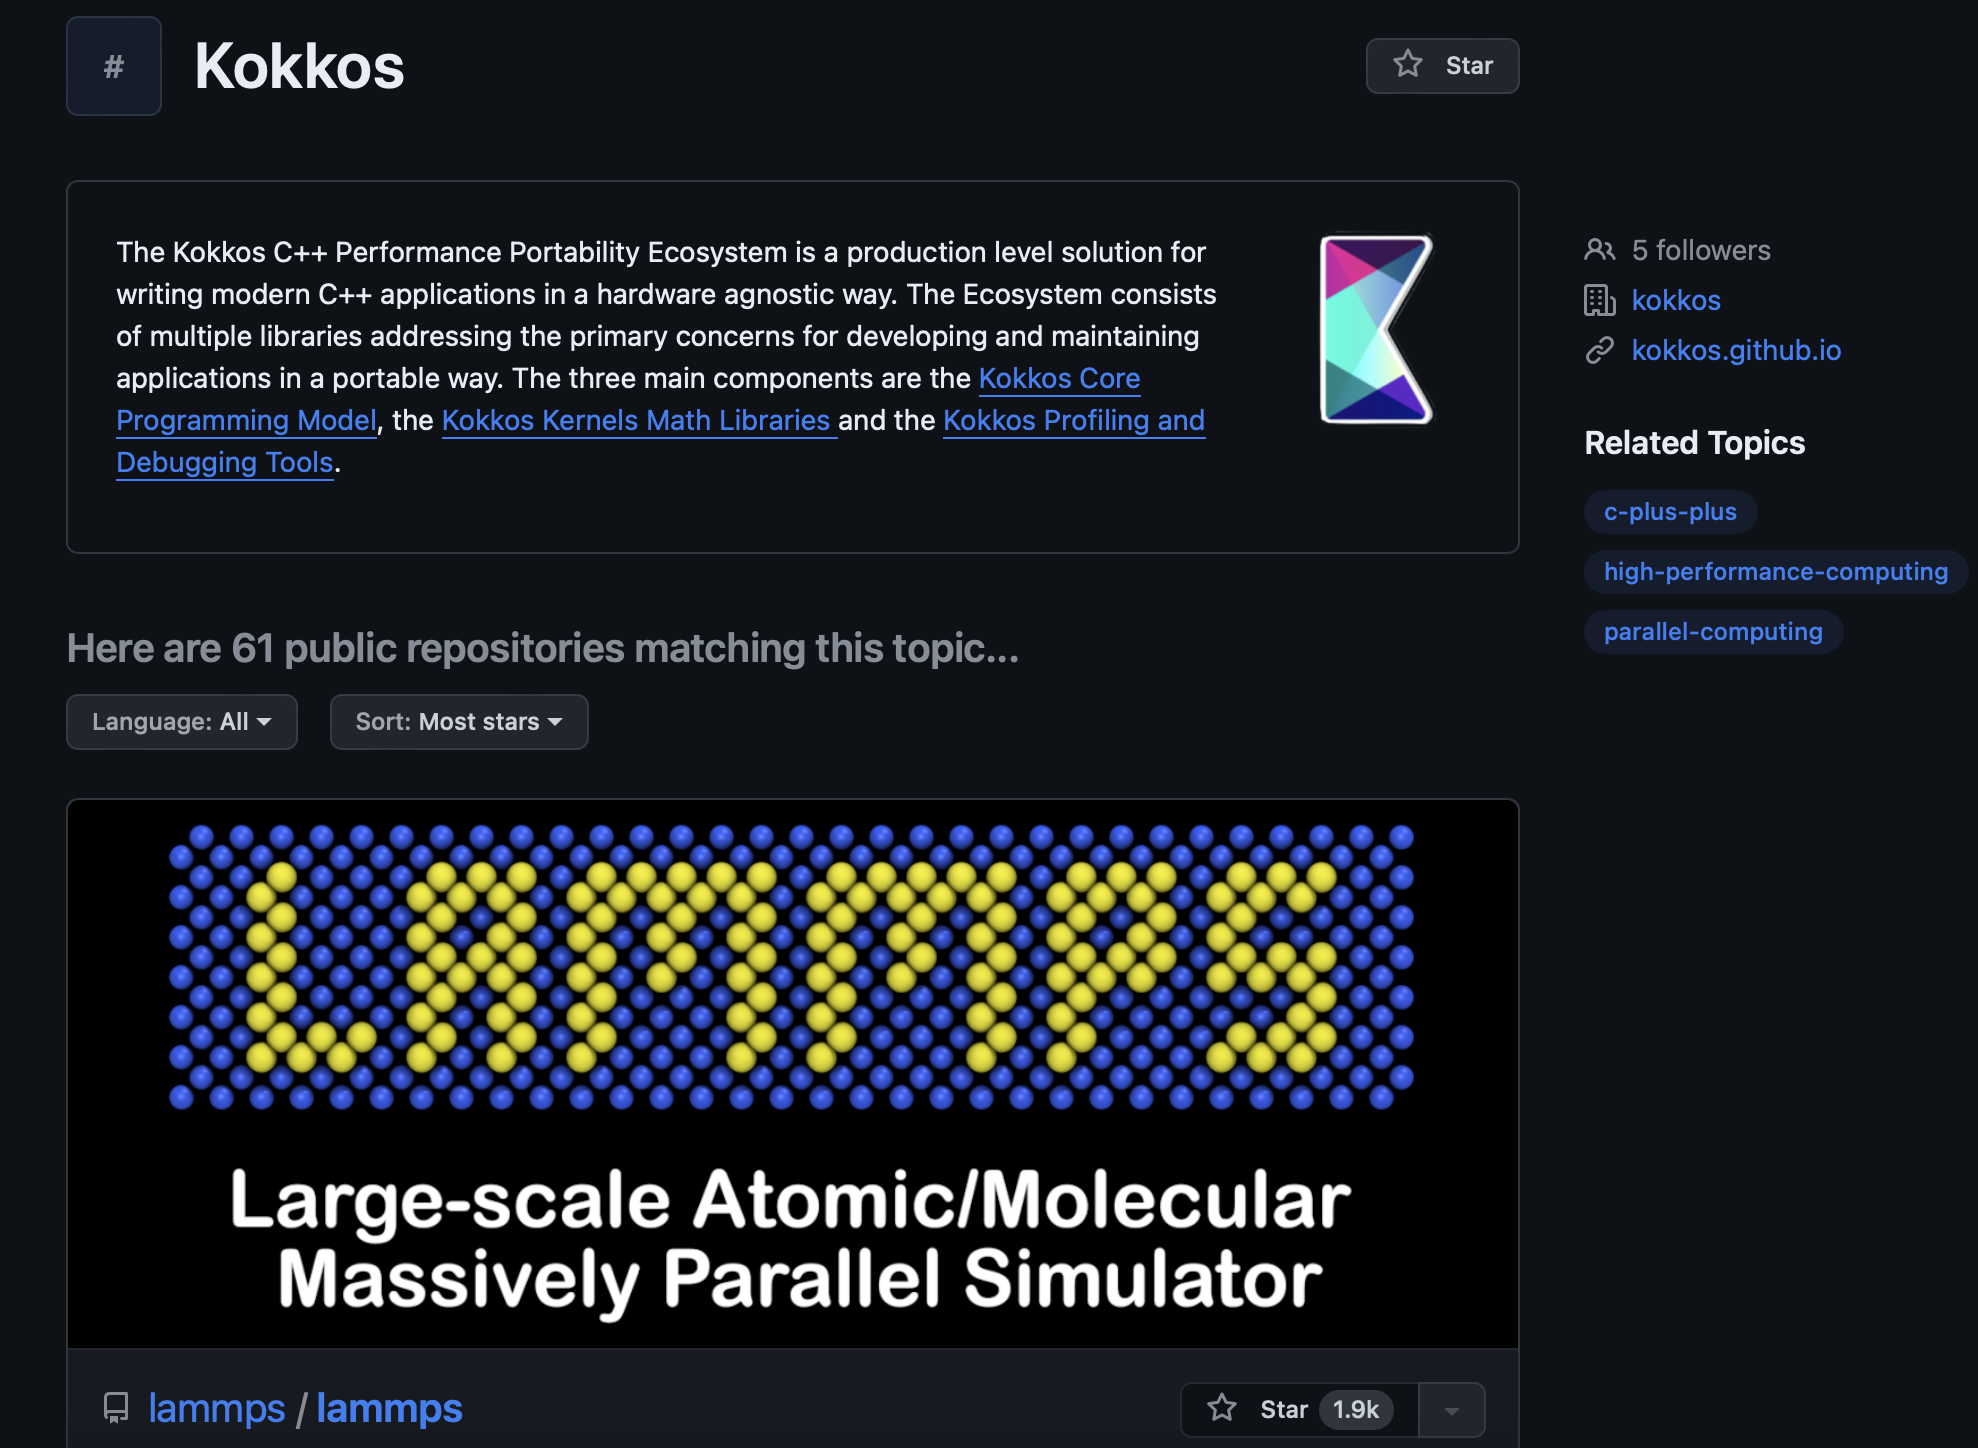
\includegraphics[width=0.9\textwidth]{4_3/kokkos-topic}
\end{frame}


%==========================================================================

\begin{frame}[fragile]

  {\Huge Organizational}

  \vspace{10pt}

  \textbf{Content:}
  \begin{itemize}
    \item HPSF and Kokkos Meeting 2025
    \item Targeting C++20 for Kokkos 5.0
    \item Makefile deprecation
  \end{itemize}

\end{frame}

%==========================================================================

\begin{frame}[fragile]{Kokkos User Group Meeting 2025}
\begin{center}
\textbf{Kokkos User Group Meeting 2025 @ HPSF Conference}
\end{center}

\begin{itemize}
\item{\textit{When:} May 5th-8th 2025}
\item{\textit{Where:} Chicago}
\item{\textit{What:} 2-days HPSF plenary + 2-days Project meetings}
\item{\textit{KUG-Content:} Focused on user experiences
\begin{itemize}
   \item{How do you leverage Kokkos?}
   \item{What are pain points?}
   \item{Kokkos-based libraries of interest to the community}
\end{itemize}
}
\end{itemize}

\vspace{10pt}

\begin{center}
\textit{Registration open now!}
\end{center}
\end{frame}

\begin{frame}[fragile]{Kokkos User Group Meeting 2025}
\begin{center}
\textbf{What to expect from KUG}
\end{center}

\begin{itemize}
  \item{Eight 90-minute sessions featuring a dynamic blend of Kokkos developers and community users}

  \begin{multicols}{2}
    \item{\textit{Day 1 Highlights:}}
      \begin{itemize}
        \item{Essential Updates}
        \item{Kokkos in Applications}
        \item{Adopting Kokkos}
        \item{Lightning Talks}
    \end{itemize}

    \columnbreak

    \item{\textit{Day 2 Highlights:}}
      \begin{itemize}
        \item{Kokkos Ecosystem}
        \item{Tuning and Performance}
        \item{Algorithms}
        \item{Panel Discussion}
    \end{itemize}
  \end{multicols}
\end{itemize}
\end{frame}

\begin{frame}[fragile]{HPSF Conference 2025}
\begin{center}
\textbf{Other reasons to go}
\end{center}

\begin{itemize}
  \item{General Poster Session}
  \item{Updates on the HPSF project}
  \item{Introduction to various working groups}
  \item{Various Panel Discussions}
  \item{Chance to meet all other members of HPSF}
  \item{...}
\end{itemize}
\end{frame}

\begin{frame}[fragile]{Other outreach}
  \begin{itemize}
    \item{HPSF will be present at \href{https://isc.app.swapcard.com/widget/event/isc-high-performance-2025/planning/UGxhbm5pbmdfMjU4NjE0MQ==}{ISC BOF 2025}}
\item{\href{https://kokkos.org/community/tea-time/}{Kokkos Tea-Time} on 2nd or 3rd Wed of the month} 
  \begin{itemize}
      \item April 16th @ 11am EST "Solomon: unified schemes for directive-based GPU offloading"
  \end{itemize}
\end{itemize}

\end{frame}


\begin{frame}[fragile]{Kokkos 5 and ISO C++20}
\begin{center}
\textbf{Kokkos 5 is comming Summer 2025}

\vspace{0.5cm}
\textbf{We will require C++20!}
\end{center}

\textit{Start preparing now:}
\begin{itemize}
  \item{Check availability of compilers on your systems}
  \item{Test with C++20 enabled: start with a CPU build}
  \item{Minimum Compiler requirements will change (more details later)}
\end{itemize}

\vspace{0.5cm}
\begin{center}
\textit{Nothing wrong for your project to require C++20 now if you feel ready!}
\end{center}
\end{frame}

\begin{frame}[fragile]{Makefile deprecation}
\begin{center}
\textbf{Makefile is officially deprecated and will be removed in the next major release}

\textit{Start preparing now:}
\begin{itemize}
  \item{Check if you can transition to CMake}
  \item{Comment on pinned issue \href{https://github.com/kokkos/kokkos/issues/7610}{7610}}
\end{itemize}
\end{center}

\end{frame}

\begin{frame}[fragile]{Open SSF Scorecard}
\begin{center}
\textbf{We reached ``passed'' on the OSSF Best Practices Program}
\href{https://www.bestpractices.dev/en/projects/9344}{www.bestpractices.dev}

\vspace{0.5cm}
\textit{This means Kokkos is continuously tracking and openly reporting the conformity with open source software practices.}
\end{center}

\end{frame}


%==========================================================================

\begin{frame}[fragile]

  {\Huge Backend Updates}

  \vspace{10pt}

  \textbf{Content:}
  \begin{itemize}
    \item Backend Updates Cuda
    \item Backend Updates HIP
    \item Backend Updates SYCL and OpenACC
  \end{itemize}

\end{frame}

%==========================================================================

\begin{frame}[fragile]{Backend Updates I}
\texttt{CUDA}
\begin{itemize}
    \item Fixed potential data race in \texttt{parallel\_reduce}
    \item Use \texttt{cudaMallocAsync} by default
    \item Bugfix when specifying non-default device ID while launching threads after initialization
    \item Deprecate \texttt{Cuda(cudaStream\_t,bool)} constructor
\end{itemize}
\end{frame}
\begin{frame}[fragile]{Backend updates II}
\texttt{HIP}
\begin{itemize}
    \item New naming convention:\\ \texttt{Kokkos\_ARCH\_VEGA90A} $\rightarrow$ \texttt{Kokkos\_ARCH\_AMD\_GFX90A}
    \item Add initial support for gfx942
    \item Add support for ROCM 5.5 and 5.6
    \item Improve reduction performance
    \item Fix potential data race in \texttt{HIP} \texttt{parallel\_reduce}
    \item Deprecate \texttt{HIP(hipStream\_t,bool)} constructor
    \item Add support for \texttt{Kokkos::Graph}
    \item Fix concurrency calculation
\end{itemize}
\end{frame}
\begin{frame}[fragile]{Backend Updates III}
\texttt{SYCL}
\begin{itemize}
    \item Enforce external \texttt{sycl::queues} to be in-order
    \item Make in-order \texttt{sycl::queues} the default via macro
    \item Improve reduction performance
    \item Allow using the \texttt{SYCL} execution space on AMD GPUs
    \item Allow sorting via native \texttt{oneDPL} to support \texttt{View}s with \texttt{stride=1}
\end{itemize}
\vfill
\texttt{OpenACC}
\begin{itemize}
    \item Add support for \texttt{clacc} compiler
\end{itemize}
\end{frame}

%==========================================================================



%==========================================================================


% Makefile and CMake support for C++23
% Update minimum compiler versions. (covered in earlier section)

\begin{frame}[fragile]{Build System Updates}
\textbf{C++ Standards Support}
\begin{itemize}
  \item \texttt{CMAKE\_CXX\_STANDARD=23} is supported
  \begin{itemize}
    \item \texttt{KOKKOS\_CXX\_STANDARD} for the Makefile
  \end{itemize}
  \item In CMake Kokkos will default to C++17 if no standard is specified
\end{itemize}
\end{frame}

%==========================================================================

% Let CMake determine OpenMP flags.
% Only add -latomic in generated GNU makefiles when OpenMPTarget backend is enabled

\begin{frame}[fragile]{Build System Updates}
\textbf{OpenMP and OpenMPTarget}
\begin{itemize}
  \item OpenMP flags are now determined by CMake's FindOpenMP
  \item Makefile: \texttt{libatomic} only linked in OpenMPTarget builds
\end{itemize}
\end{frame}

%==========================================================================

% Do not add -cuda to the link line with NVHPC compiler when the CUDA backend is not actually enabled
% Kokkos_ENABLE_CUDA_LAMBDA now ON by default with NVCC
% Fix enabling of relocatable device code when using CUDA as CMake language
% Fix cmake configuration with CUDA 12

\begin{frame}[fragile]{Build System Updates}
\textbf{CUDA}
\begin{itemize}
  \item \texttt{Kokkos\_ENABLE\_CUDA\_LAMBDA} set to \texttt{ON} by default
  \item Fixes to RDC flags when using CMake CUDA language
  \item Fixed CUDA 12 when using \texttt{nvcc\_wrapper} with CMake
  \item Fixes to using NVHPC as a compiler when CUDA is not enabled
\end{itemize}
\end{frame}

%==========================================================================



%==========================================================================

\begin{frame}[fragile]{sort\_by\_key}

\textbf{Introduced sort\_by\_key to dispatch to optimized vendor libraries}

\vspace{10pt}

\begin{code}
  ExecutionSpace exec_space;
  Kokkos::View<int*> keys("keys", n);
  Kokkos::View<float*> values("values", n);
  Kokkos::Experimental::sort_by_key(exec_space, keys, values);
\end{code}

\vspace{10pt}

\begin{itemize}
  \item 1D views only
  \item Sizes of \texttt{keys} and \texttt{values} must match
  \item Both \texttt{keys} and \texttt{values} are modified
  \item Dispatches to vendor libraries (Thrust, rocThrust, oneDPL) when available
\end{itemize}

\end{frame}

%==========================================================================


%==========================================================================

\begin{frame}[fragile]

  {\Huge General Enhancements}

  \vspace{10pt}

\end{frame}

%==========================================================================
\begin{frame}[fragile]{\texttt{Array}}

Improve \texttt{Array} facility to align further with \texttt{std::array}
\begin{itemize}
\item Add \texttt{to\_array()}
\begin{code}
char a[] = { 'f', 'o', 'o', '\0' };
auto b = Kokkos::to_array(a);                // Kokkos::Array<char, 4>

auto c = Kokkos::to_array({0, 2, 1, 3});     // Kokkos::Array<int, 4>
auto d = Kokkos::to_array<long>({0, 1, 3});  // Kokkos::Array<long, 3>;
\end{code}
\item Provide \texttt{kokkos\_swap(Array<T, N>\&, Array<T, N>\&)} specialization
\item Make \texttt{Array<T, N>} equality comparable
\begin{code}
Kokkos::Array<int, 2> e = /* ... */;
Kokkos::Array<int, 2> f = /* ... */;

KOKKOS_ASSERT((e == f) != (e != f));
\end{code}
\end{itemize}

\end{frame}

%==========================================================================

\begin{frame}[fragile]{\texttt{TeamPolicy} CTAD}
\begin{itemize}
\item Added CTAD deduction guides for \texttt{TeamPolicy}
\begin{code}
TeamPolicy()                                -> TeamPolicy<>;
TeamPolicy(int, ...)                        -> TeamPolicy<>;
TeamPolicy(DefaultExecutionSpace, int, ...) -> TeamPolicy<>;

static_assert(!is_same_v<SomeExecutionSpace, DefaultExecutionSpace>);
TeamPolicy(SomeExecutionSpace, int, ...)    -> TeamPolicy<SomeExecutionSpace>;

\end{code}
\end{itemize}

\end{frame}

%==========================================================================

% \begin{frame}[fragile]{Structured binding support for Kokkos::complex}

\begin{frame}[fragile]{Structured binding support for \texttt{complex}}
\begin{itemize}
\item Added tuple protocol to \texttt{complex} for structured binding support
  \begin{itemize}
  \item Based on structured binding support for \texttt{std::complex} added to C++26
  \item Add Tuple Protocol to \texttt{complex}
  \item[]   \url{https://wg21.link/P2819R2} 
  \end{itemize}
\begin{code}
Kokkos::complex<double> z(11., 13.);
auto&[r, i] = z;
Kokkos::kokkos_swap(r, i);
KOKKOS_ASSERT(r == 13. && i == 11.);
\end{code}
\end{itemize}

\end{frame}



% \end{frame}

%==========================================================================
\begin{frame}[fragile]{Add converting constructor in Kokkos::RandomAccessIterator}

\begin{itemize}
\item Harmonize \texttt{View} and (internal) random access iterator convertibility
\end{itemize}

\begin{code}[keywords={Convertibility rules}]
Kokkos::View<int *> x;
Kokkos::View<const int *> const_y(x); // compiles
//Kokkos::View<int *> y(const_x); // compiler error

auto x_it = begin(x);
decltype(begin(const_y)) const_it = x_it; // previously did not compile
\end{code}

\end{frame}
%==========================================================================
\begin{frame}[fragile]{Add a check precondition non-overlapping ranges for the adjacent\_difference algorithm}
\begin{itemize}
\item Disallow the overlapping of source and destination iterators (in debug mode). See \url{https://eel.is/c++draft/numeric.ops#adjacent.difference-8}
\item DO NOT check overlapping if the source and destination iterators are constructed from a single multidimensional view and the strides of these iterators are not identical
\end{itemize}

\begin{code}[keywords={Check overlaps in debug mode}]
// Case 0 No longer allowed (Source and destination iterators are the same)
Kokkos::View<double*> a("A",N0);
auto res1 = KE::adjacent_difference("label", exespace(), a, a, args...);

// Case 1 Still allowed (b0/b1 iterates over even/odd numbers only)
Kokkos::View<double[2]*> b("B",N0);
auto sub_b0 = Kokkos::subview(b, 0, Kokkos::ALL);
auto sub_b1 = Kokkos::subview(b, 1, Kokkos::ALL);
auto sub_first_b0 = KE::begin(sub_b0);  // 0, 2, 4, ...
auto sub_first_b1 = KE::begin(sub_b1); // 1, 3, 5, ...
auto res2 = KE::adjacent_difference("label", exespace(),
            sub_first_b0, sub_first_b1, args...);
\end{code}

\end{frame}
%==========================================================================
% \begin{frame}[fragile]{Improve compile-times with Kokkos_ENABLE_DEBUG_BOUNDS_CHECK in Cuda}

% \end{frame}
%==========================================================================

\begin{frame}[fragile]{SIMD: Allow flexible vector width for 32 bit types}

\textbf{Use full vector width for 32 bit data types}
\begin{itemize}
  \item The vector width of \texttt{Kokkos::simd} was determined based on 64 bit data types in available vector registers
  \item For 32 bit data types, Abi can be specified to use larger vector width
\end{itemize}

\begin{code}[keywords={simd}]
  {
    // For AVX512
    using namespace Kokkos::Experimental;
    using native_type      = native_simd<float>;
    using simd_type        = simd<float, simd_abi::avx512_fixed_size<8>>;
    using simd_larger_type = simd<float, simd_abi::avx512_fixed_size<16>>; 

    static_assert(simd_type::size()   == native_type::size());
    static_assert(simd_type::size()*2 == simd_larger_type::size());
  }
\end{code}

Applied for: AVX2, AVX512, NEON

\end{frame}

%==========================================================================
\begin{frame}[fragile]{Host: Use unlikely attribute when reference counting views on host backends}
  \begin{itemize}
    \item We use \texttt{unlikely} attribute from C++20 to improve reference counting in views on host backends.
    \item This only impacts LLVM compilers.
  \end{itemize}

\end{frame}
%==========================================================================


%==========================================================================

\begin{frame}[fragile]

  {\Huge Querying the Number of Devices}

  \vspace{10pt}

	\textbf{Content:}
  \begin{itemize}
    \item Runtime function for querying the number of devices
    \item Device ID consistency with \texttt{KOKKOS\_VISIBLE\_DEVICES}
  \end{itemize}

\end{frame}

%==========================================================================

\begin{frame}[fragile]{Querying the number of devices}

\textbf{A runtime function to query the number of devices}
\bigskip

\texttt{[[nodiscard]] int Kokkos::num\_devices() noexcept {...}}
\vspace{10pt}

\begin{itemize}
	\item Callable before \texttt{Kokkos::initialize()}
	\item Returns the device count based on visible devices
	\item Returns -1 if no GPU backend is enabled
	\item Replaces \texttt{{Cuda,HIP}::detect\_device\_count()}
\end{itemize}

\end{frame}

%==========================================================================

\begin{frame}[fragile]{Kokkos::device\_id() consistency}

\textbf{Fixed a defect in \texttt{Kokkos::device\_id()}}
\bigskip

\texttt{KOKKOS\_VISIBLE\_DEVICES} were not being considered for \texttt{Kokkos::device\_id()}.
\vspace{10pt}

\begin{table}[]
\begin{tabular}{l|llll}
\multicolumn{1}{c|}{\textbf{initialization settings}} & \multicolumn{1}{c}{\textbf{Pre-4.3}} & \multicolumn{1}{c}{\textbf{4.3}} &  &  \\ \hline
\textless{}none\textgreater{}                         & 0                                    & 0                                &  &  \\
device\_id=1                                          & 1                                    & 1                                &  &  \\
KOKKOS\_VISIBLE\_DEVICES=0                            & 0                                    & 0                                &  &  \\
KOKKOS\_VISIBLE\_DEVICES=3                            & 3                                    & 0                                &  &  \\
KOKKOS\_VISIBLE\_DEVICES=1,0                          & 1                                    & 0                                &  &  \\
device\_id=1 KOKKOS\_VISIBLE\_DEVICES=1,0             & 0                                    & 1                                &  & 
\end{tabular}
\end{table}

\end{frame}

%==========================================================================


%==========================================================================

\begin{frame}[fragile]

  {\Huge Kokkos SIMD}

  \vspace{10pt}

  \textbf{Content:}
	\begin{itemize}
		\item \texttt{simd\_flags}
		\item \texttt{vector\_aligned\_tag}
	\end{itemize}

\end{frame}

%==========================================================================

\begin{frame}[fragile]{simd\_flags}

\textbf{Introduced \texttt{simd\_flags} to match latest ISO C++ proposal on \texttt{std::simd}}

\vspace{10pt}

\texttt{template <typename... Flags> struct simd\_flags}

\vspace{10pt}

\begin{itemize}
	\item \texttt{element\_aligned\_tag <-> simd\_flag\_default}
	\item \texttt{vector\_aligned\_tag <-> simd\_flag\_aligned}
\end{itemize}

\vspace{10pt}
\texttt{simd\_flags} are used in:
\begin{itemize}
  \item \texttt{template <class U, class Flags> void copy\_from(const U* mem, Flags flags)}
  \item \texttt{template <class U, class Flags> void copy\_to(U* mem, Flags flags)}
\end{itemize}

\end{frame}

%==========================================================================

\begin{frame}[fragile]{simd\_flags}

\begin{code}[keywords={simd_flags}]
void init_var() {
  constexpr size_t alignment =
    Kokkos::Experimental::native_simd::size() * sizeof(DataType);

  alignas(alignment) DataType const src[N] = { ... };

  simd_type var;
  var.copy_from(src, Kokkos::Experimental::simd_flag_aligned);

  ...
}
\end{code}

\end{frame}

%==========================================================================

%==========================================================================

\begin{frame}[fragile]

  {\Huge Bitset Constructor Update}

\end{frame}

%==========================================================================

\begin{frame}[fragile]{Bitset constructor update}

\texttt{Bitset(unsigned arg\_size = 0u)}
\vspace{10pt}
\begin{itemize}
	\item A \texttt{Bitset} constructor with a default size of \texttt{Bitset} was making a deferred constructor call.
	\item Caused an unnecessary memory allocation when \texttt{Bitset} was constructed with the default size of 0.
\end{itemize}

\vspace{10pt}

Refactored to no longer have the default argument and use a defaulted default \texttt{Bitset} constructor instead.

\end{frame}

%==========================================================================

%==========================================================================

\begin{frame}[fragile]

  {\Huge Random Number Generator}

\end{frame}


\begin{frame}[fragile]{Random Number Generator}
\texttt{Normal distribution improvements}
\begin{itemize}
\item Replace Marsaglia polar method with Box-Muller method 
\item Box-Muller contains no branching/looping, single code path, ideal for GPU
\item Kokkos performance on GPU, Nvidia: 
\begin{itemize}
\item ~20\% faster for 64 bit version
\item ~60\% faster for 1024 bit version
\end{itemize}
\end{itemize}
\end{frame}

%==========================================================================


%==========================================================================

\begin{frame}[fragile]

  {\Huge New Public Headers}
  
    \vspace{10pt}

  \textbf{Content:}
    \begin{itemize}
        \item \texttt{Kokkos\_Clamp.hpp}
        \item \texttt{Kokkos\_MinMax.hpp}
    \end{itemize}


\end{frame}

%==========================================================================

\begin{frame}[fragile]{Kokkos\_Clamp.hpp}

\begin{code}[keywords={Clamp}]

// bounded value

template<class T>
constexpr const T& clamp(const T& value, const T& low, const T& high);

template<class T, class ComparatorType>
constexpr T const& clamp(const T& value, const T& low, const T& high,
                         ComparatorType comp);

\end{code}

\end{frame}

%==========================================================================

\begin{frame}[fragile]{Kokkos\_MinMax.hpp Max}

\begin{code}[keywords={MinMax}]

// max

template <class T>
constexpr const T& max(const T& a, const T& b);
  
template <class T, class ComparatorType>
constexpr const T& max(const T& a, const T& b, ComparatorType comp);
  
template <class T>
constexpr T max(std::initializer_list<T> ilist); 
      
template <class T, class Compare>
constexpr T max(std::initializer_list<T> ilist, Compare comp); 


\end{code}

\end{frame}

%==========================================================================
\begin{frame}[fragile]{Kokkos\_MinMax.hpp Min}

\begin{code}[keywords={MinMax}]

// min

template <class T>
constexpr const T& min(const T& a, const T& b);

template <class T, class ComparatorType>
constexpr const T& min(const T& a, const T& b,ComparatorType comp);

template <class T>
constexpr T min(std::initializer_list<T> ilist);

template <class T, class Compare>
constexpr T min(std::initializer_list<T> ilist, Compare comp);

\end{code}

\end{frame}

%==========================================================================
\begin{frame}[fragile]{Kokkos\_MinMax.hpp MinMax}

\begin{code}[keywords={MinMax}]

// minmax

// minmax
template <class T>
constexpr Kokkos::pair<const T&, const T&> minmax(const T& a, const T& b);

template <class T, class ComparatorType>
constexpr Kokkos::pair<const T&, const T&> minmax(const T& a, const T& b,
                                                  ComparatorType comp);

template <class T>
constexpr Kokkos::pair<T, T> minmax(std::initializer_list<T> ilist);

template <class T, class Compare>
constexpr Kokkos::pair<T, T> minmax(std::initializer_list<T> ilist, Compare comp);

\end{code}

\end{frame}

%==========================================================================


%==========================================================================

\begin{frame}[fragile]

  {\Huge Compile-Time Argument Deduction (CTAD / Deduction Guides)}
  
    \vspace{10pt}

  \textbf{Content:}
    \begin{itemize}
        \item What are deduction guides?
        \item \texttt{Kokkos::Array} deduction guide
        \item \texttt{Kokkos::RangePolicy} deduction guides
        \item \texttt{Kokkos::MDRangePolicy} deduction guides
    \end{itemize}


\end{frame}

%==========================================================================

\begin{frame}[fragile]{CTAD / Deduction Guides}

\begin{itemize}
\item C++17
\item Usability Improvement
\item Deduces class template parameters from types and/or number of parameters passed to constructors
\item Eliminates need to specify template parameters when declaring automatic variables
\end{itemize}

\end{frame}

%==========================================================================

\begin{frame}[fragile]{Array Deduction Guide}

\begin{code}[keywords={Array}]
// Kokkos::Array<double, 3>
Kokkos::Array a4{3.0, 1.0, 4.0};	
\end{code}

\begin{itemize}
\item matches \texttt{std::array} deduction guide
\end{itemize}

\end{frame}

%==========================================================================

\begin{frame}[fragile]{RangePolicy Deduction Guides}

\begin{code}[keywords={RangePolicy}]

int64_t work_begin   = /* ... */;  // conversions as well
int64_t work_end     = /* ... */;  // conversions as well
Kokkos::ChunkSize cs = /* ... */;  // conversions as well
Kokkos::DefaultExecutionSpace des; // conversions as well
SomeExecutionSpace ses;            // different from Kokkos::DefaultExecutionSpace

// Kokkos::RangePolicy<>
Kokkos::RangePolicy rp0;
Kokkos::RangePolicy rp1(work_begin, work_end);
Kokkos::RangePolicy rp2(work_begin, work_end, cs);
Kokkos::RangePolicy rp3(des, work_begin, work_end);
Kokkos::RangePolicy rp4(des, work_begin, work_end, cs);

// Kokkos::RangePolicy<SomeExecutionSpace>
Kokkos::RangePolicy rp5(ses, work_begin, work_end);
Kokkos::RangePolicy rp6(ses, work_begin, work_end, cs);

\end{code}

\end{frame}

%==========================================================================

\begin{frame}[fragile]{MDRangePolicy initializer\_list Deduction Guides}

\begin{code}[keywords={MDRangePolicy initializer_list}]

Kokkos::DefaultExecutionSpace des;
SomeExecutionSpace ses;            // different from Kokkos::DefaultExecutionSpace
int64_t i;

// Kokkos::MDRangePolicy<Kokkos::Rank<5>>
Kokkos::MDRangePolicy pl0({1, 2, 3, 4, 5}, {1, 2, 3, 4, 5});
Kokkos::MDRangePolicy pl1({1, 2, 3, 4, 5}, {1, 2, 3, 4, 5}, { i });
Kokkos::MDRangePolicy pl2(des, {1, 2, 3, 4, 5}, {1, 2, 3, 4, 5});
Kokkos::MDRangePolicy pl3(des, {1, 2, 3, 4, 5}, {1, 2, 3, 4, 5}, { i });

// Kokkos::MDRangePolicy<SomeExecutionSpace, Kokkos::Rank<5>>
Kokkos::MDRangePolicy pl4(ses, {1, 2, 3, 4, 5}, {1, 2, 3, 4, 5});
Kokkos::MDRangePolicy pl5(ses, {1, 2, 3, 4, 5}, {1, 2, 3, 4, 5}, { i });

\end{code}

\end{frame}

%==========================================================================

\begin{frame}[fragile]{MDRangePolicy C Array Deduction Guides}

\begin{code}[keywords={MDRangePolicy C Array}]

Kokkos::DefaultExecutionSpace des;
SomeExecutionSpace ses;            // different from Kokkos::DefaultExecutionSpace
int cbegin[3];
int cend[3];
int64_t ctiling[2];

// Kokkos::MDRangePolicy<Kokkos::Rank<3>>
Kokkos::MDRangePolicy pc0(cbegin, cend);
Kokkos::MDRangePolicy pc1(cbegin, cend, ctiling);
Kokkos::MDRangePolicy pc2(des, cbegin, cend);
Kokkos::MDRangePolicy pc3(des, cbegin, cend, ctiling)

// Kokkos::MDRangePolicy<SomeExecutionSpace, Kokkos::Rank<3>>
Kokkos::MDRangePolicy pc4(ses, cbegin, cend);
Kokkos::MDRangePolicy pc5(ses, cbegin, cend, ctiling);

\end{code}

\end{frame}

%==========================================================================
\begin{frame}[fragile]{MDRangePolicy Array Deduction Guides}

\begin{code}[keywords={MDRangePolicy Kokkos::Array}]

Kokkos::DefaultExecutionSpace des;
SomeExecutionSpace ses;            // different from Kokkos::DefaultExecutionSpace
Kokkos::Array<int, 2> abegin;
Kokkos::Array<int, 2> aend;
Kokkos::Array<int64_t, 2> atiling;

// Kokkos::MDRangePolicy<Kokkos::Rank<2>>
Kokkos::MDRangePolicy pa0(abegin, aend);
Kokkos::MDRangePolicy pa1(abegin, aend, atiling);
Kokkos::MDRangePolicy pa2(des, abegin, aend);
Kokkos::MDRangePolicy pa3(des, abegin, aend, atiling)

// Kokkos::MDRangePolicy<SomeExecutionSpace, Kokkos::Rank<2>>
Kokkos::MDRangePolicy pa4(ses, abegin, aend);
Kokkos::MDRangePolicy pa5(ses, abegin, aend, atiling);

\end{code}

\end{frame}

%==========================================================================

%==========================================================================

\begin{frame}[fragile]

  {\Huge Misc. Algorithmic Improvements/Fixes}

\end{frame}

\begin{frame}[fragile]{Misc. Algorithmic Improvements/Fixes}
\begin{itemize}
\item Kokkos\textunderscore Unique.hpp
\begin{itemize}
\item Allocate temporary view with provided execution space
\item Remove unnecessary init for temporary view during construction
\end{itemize}
\item Kokkos\_RemoveIf.hpp
\begin{itemize}
\item Allocate temporary view with provided execution space
\item Remove unnecessary init for temporary view during construction
\item Remove unnecessary predicate evaluation
\begin{itemize}
\item[] Important since predicate can be arbitrarily expensive
\end{itemize}
\end{itemize}
\end{itemize}
\end{frame}

%==========================================================================


%==========================================================================

\begin{frame}[fragile]

  {\Huge Range/MDRangePolicy Updates}

  \vspace{10pt}

  \textbf{Content:}
  \begin{itemize}
    \item Begin and end bounds check
    \item Unsafe implicit conversion check
    \item RangePolicy variadic constructor removal 
  \end{itemize}

\end{frame}

%==========================================================================

\begin{frame}[fragile]{Bounds Check}

\textbf{Asserts that the upper bound is greater than the lower bound}

\vspace{10pt}
\begin{code}[keywords={BoundsCheck}]
  Kokkos::RangePolicy<> policy(100, 90);
  Kokkos::MDRangePolicy<Kokkos::Rank<2>> policy({100, 100}, {100, 90});
\end{code}
\vspace{10pt}

Aborts with:
\textit{Kokkos::MDRangePolicy bounds error: The lower bound (100) is greater than its upper bound (90) in dimension ...}
\vspace{10pt}

\begin{itemize}
	\item If \texttt{KOKKOS\_ENABLE\_DEPRECATED\_CODE\_4} is not defined, aborts.
	\item Else if \texttt{KOKKOS\_ENABLE\_DEPRECATION\_WARNINGS} is defined, outputs to \texttt{std::cerr}.
\end{itemize}

\end{frame}

%==========================================================================

\begin{frame}[fragile]{Unsafe Implicit Conversion Check}

\textbf{Checks for unsafe implicit index type conversions during RangePolicy construction}
\begin{itemize}
  \item Narrowing conversions
  \item Sign conversions
\end{itemize}
\vspace{10pt}

Aborts with:
\textit{Kokkos::RangePolicy bound type error: an unsafe implicit conversion is performed on a bound (...)}
\textit{which may not preserve its original value.}
\vspace{10pt}

\begin{itemize}
	\item If \texttt{KOKKOS\_ENABLE\_DEPRECATED\_CODE\_4} is not defined, aborts.
	\item Else if \texttt{KOKKOS\_ENABLE\_DEPRECATION\_WARNINGS} is defined, outputs to \texttt{std::cerr}.
\end{itemize}

\end{frame}

%==========================================================================

\begin{frame}[fragile]{RangePolicy constructor cleanup}

\textbf{Removed RangePolicy variadic constructors}
\bigskip

\begin{code}[keywords={RangePolicyConstructorCleanup}]
template<class ...InitArgs>
RangePolicy(const IndexType&, const IndexType&, const InitArgs...)
template<class ...InitArgs>
RangePolicy(const ExecutionSpace&, const IndexType&, const IndexType&,
            const InitArgs...)

RangePolicy(const IndexType&, const IndexType&, const ChunkSize)
RangePolicy(const ExecutionSpace&, const IndexType&, const IndexType&,
            const ChunkSize)
\end{code}

\vspace{10pt}
\texttt{template <class... Args> inline void set(Args...)} is deprecated in favor of

\texttt{inline RangePolicy\& set\_chunk\_size(int chunk\_size)}.

\end{frame}

%==========================================================================

%==========================================================================

\begin{frame}[fragile]

  {\Huge Bug Fixes}

  \vspace{10pt}

\end{frame}

%==========================================================================

% Examples

% note: always keep the [fragile] for your frames!

%\begin{frame}[fragile]{Example list}
%  \begin{itemize}
%      \item Item 1
%      \item Item 2 with some \texttt{code}
%      \begin{itemize}
%        \item Sub-item 2.1
%        \item Sub-item 2.2
%      \end{itemize}
%  \end{itemize}
%\end{frame}

%\begin{frame}[fragile]{Example code}
%    \begin{code}[keywords={std}]
%        #include <iostream>
%        
%        int main() {
%            std::cout << "hello world\n";
%        }
%    \end{code}
%\end{frame}

%\begin{frame}[fragile]{Example table}
%    \begin{center}
%        \begin{tabular}{l|l}
%            a & b \\\hline
%            c & d
%        \end{tabular}
%    \end{center}
%\end{frame}

%==========================================================================

\begin{frame}[fragile]{General Bug Fixes}
    \begin{itemize}
      \item Fix a memory leak from an early exit when using \texttt{--kokkos-tools-help} % 8074
      \item Add missing fences for async Random init with unified memory % 8105
      \item More robust checks on subview constructor % #8210
        \begin{code}[keywords={std}]
View<T**, LayoutLeft> a(N,N);

// Previously allowed, but data should have strided access.
View<T*, LayoutLeft> sub_a(a, 1, ALL); // Runtime Error
        \end{code}

    \end{itemize}
\end{frame}

%==========================================================================

\begin{frame}[fragile]{General Bug Fixes}
  \begin{itemize}
    \item SIMD:
    \begin{itemize}
      \item Fix compile errors with \texttt{Kokkos\_ARCH\_NATVE=ON} % 7912
      \item Fix fallback simd masked reductions using incorrect identity elements % 8115
    \end{itemize}
    \item Compilers:
    \begin{itemize}
      \item Apply a workaround for a segfault issue in \texttt{SharedAllocationTracker} with gcc 12.2, 12.3 and 12.4 % 8223
      \item Fix compiling with C++23 supported compilers that provide an mdspan implementation % #8234
    \end{itemize}
  \end{itemize}
\end{frame}

%==========================================================================

\begin{frame}[fragile]{Backend Bug Fixes}
    \begin{itemize}
        \item HPX: fix to constrain hpx\_thread\_buffer size used with TeamPolicy setup % #8147
        \item HIP and SYCL:
        \begin{itemize}
          \item A \texttt{MDRangePolicy} of rank 4 or more would be incorrectly iterated, leading to some iterations being evaluated more than once for large enough loops % 7880
        \end{itemize}
        \item HIP:
        \begin{itemize}
          \item \texttt{ConstantMemory} launch mechanism would sporadically fail due to \texttt{hipEventSynchronize} error % 8094
          \item Fix launch of intermediate size functors in graph % #8188
        \end{itemize}
        \item Serial: memory leak in internal instance data % 8042
        \item OpenMP Target and OpenACC: An out-of-bounds access would occur in \texttt{Random\_UniqueIndex} under certain circumstances % 8077
    \end{itemize}
\end{frame}




%==========================================================================

\begin{frame}[fragile]

  {\Huge Potentially Breaking Changes}
  
    \vspace{10pt}

\end{frame}

%==========================================================================

\begin{frame}[fragile]{Breaking Changes 1/1}

\begin{itemize}

\item Dropped \texttt{Array} special treatment in \texttt{View}
  \begin{itemize}
  \item was treated as an extra compile-time dimension in the view
  \item now able to construct unmanaged view of arrays
  \end{itemize}

\item Got rid of \texttt{Experimental::RawMemoryAllocationFailure}
  \begin{itemize}
  \item no known usage
  \item internally catching them and rethrowing regular \texttt{std::runtime} exceptions
  \end{itemize}

\item Bug fix for thread safety can lead to deadlocks if user code violates Kokkos sematics
      (see \textbf{Bug Fixes - Thread Safety} and \textbf{View of Views})

\end{itemize}

\end{frame}


%==========================================================================

\begin{frame}[fragile]

  {\Huge Deprecations}
  
    \vspace{10pt}

\end{frame}

\begin{frame}[fragile]{Deprecations}
\begin{itemize}
\item Deprecated allocation step inside \texttt{deep\_copy(UnorderedMap,UnorderedMap)}
  \begin{itemize}
    \item[] Maps now must have the same capacity to \texttt{deep\_copy}
  \end{itemize}
\item Deprecated implicit conversions of integers to \texttt{ChunkSize}
\begin{itemize}
  \item[] Behavior only introduced in 4.3
\end{itemize}
\item Deprecated implicit conversions to all execution spaces
\end{itemize}

\end{frame}

%==========================================================================

\begin{frame}[fragile]{Deprecate \texttt{Array<...,Proxy>} Argument}
\begin {itemize}
\item Deprecated trailing \texttt{Proxy} template argument in \texttt{Kokkos::Array}
\begin{code}
// DEPRECATED
// template <typename T = void,
//           size_t N = KOKKOS_INVALID_INDEX,
//           typename Proxy = void>
template <typename T, size_t N>
struct Array { /* ... */ };
\end{code}
  \begin{itemize}
    \item Deprecates \textit{non-owning, dynamically sized} \texttt{contiguous/strided} functionality
    \item More in line with (always) \textit{owning} \& \textit{statically sized} \texttt{std::array}
  \end{itemize}
\end{itemize}
\end{frame}

%==========================================================================

\begin{frame}[fragile]{Deprecate \texttt{is\_layouttiled}}
\begin {itemize}
\item Removed \texttt{Kokkos::Experimental::LayoutTiled} class template
  \begin{itemize}
  \item Never useable
  \end{itemize}
\item Deprecated \texttt{is\_layouttiled} trait
  \begin{itemize}
  \item Not useful, but no rush to remove it
  \end{itemize}
\item Deprecated \texttt{Kokkos::layout\_iterate\_type\_selector}
  \begin{itemize}
  \item Not useful outside of Kokkos implementation
  \end{itemize}
\end{itemize}
\end{frame}

%==========================================================================
\begin{frame}[fragile]{Deprecate \texttt{pair<T,void>}}
\begin {itemize}
\item Deprecated specialization of \texttt{Kokkos::pair} for a single element
\begin{code}
// DEPRECATED
// template <typename T>
// struct pair<T, void> { /* ... */ };
\end{code}
  \begin{itemize}
  \item Never supported in \texttt{std::pair}
  \item Never documented
  \item Never tested
  \item No known usage
  \end{itemize}
\end{itemize}
\end{frame}

%==========================================================================



%==========================================================================

\begin{frame}[fragile]

  \vspace{10pt}

  \textbf{How to Get Your Fixes and Features into Kokkos}
  \newline
  \begin{itemize}
    \item Fork the Kokkos repo (https://github.com/kokkos/kokkos)
    \item Make topic branch from \textit{develop} for your code
    \item Add tests for your code
    \item Create a Pull Request (PR) on the main project \textit{develop}
    \item Update the documentation (https://github.com/kokkos/kokkos-core-wiki) if your code changes the API
    \item Get in touch if you have any questions (https://kokkosteam.slack.com)
  \end{itemize}

\end{frame}

%==========================================================================

\end{document}
